\begin{flushright}
    \textit{Лекция 15 (от 26.10)}
\end{flushright}
$f$ мероморфна~--- тогда существует $\left\{ z_k \right\}_{n=1}^{\infty}$~---
полюсы $m_k$ порядков.
\\
Тогда $\exists \os{\circ}{B}_{\delta_k}(z_k)$, где ряд Лорана
\begin{equation}\label{(19.2)}
    f(z) = \frac{c^k_{-m_k}}{(z-z_k)^{m_k}} + \dots + \frac{c^k_{-1}}{z-z_k} + c_0^k= c_1^k(z-z_k) + \dots
\end{equation}
а его главная часть
\begin{equation}\label{(19.3)}
    q_k(z) = \frac{c^k_{-m_k}}{(z-z_k)^{m_k}} + \dots + \frac{c^k_{-1}}{z-z_k}
\end{equation}
\theorem
Пусть $f$ мероморфна, $\infty$~--- УОТ или полюс этой функции. Тогда $f$
рациональна.
\pr
$\left\{ z_k \right\}$~--- полюсы $m_k$ порядка. В силу изолированности $\infty$
набор полюсов конечен; пусть $k \in \left\{ 1, \dots, l \right\}$.
\\
$\infty$~--- УОТ или полюс; главная часть ряда Лорана в окрестности $\infty$
будет иметь вид
\begin{align*}
  & q_0 = c_1z+\dots +c_nz^n
\end{align*}
Из \eqref{(19.3)} получим $q_k(z)$ для любого $k$.
\\
Тогда
\begin{equation}\label{(19.4)}
    r(z) = f(z) - \sum_{k=0}^lq_k(z)
\end{equation}
Заметим, что $\forall k$ $r(z)$ имеет в $z_k$ устранимую особую точку. Эта
функция, доопределенная по непрерывности, будет регулярной в $\CC$ и
ограниченной на бесконечности, а значит, по теореме Лиувилля $r(z) \equiv a_0$.
Тогда из \eqref{(19.4)} получим
\begin{align*}
  & f(z) = a_0 + \sum_{k=0}^lq_k(z)
\end{align*}
а значит, $f$ рациональна.
\Def
Совокупность замкнутых простых кусочно гладких кривых $\left\{ \Gamma_n
\right\}_{n=1}^\infty$ называется \textbf{правильной}, если
\begin{itemize}
    \item $\forall n \in \NN$ область $D_n$, ограниченная $\Gamma_n$, содержится
    в области $D_{n+1}$, ограниченной $\Gamma_{n+1}$, причем $0 \in D_1$;
    \item $d_n = \min \left\{ \left| z \right| : z \in \Gamma_n \right\}
    \Rightarrow \dst \lim_{n \to \infty}d_n = \infty$;
    \item $\exists A > 0: \ \forall n \in \NN \ l_n \leq Ad_n$, где $l_n  =
    l(\Gamma_n)$.
\end{itemize}
\example
Вложенные окружности, вложенные квадраты с центром в точке $0$.
\theorem (Коши)
Пусть $f$ мероморфна и существует правильная совокупность $\left\{ \Gamma_n
\right\}_{n=1}^\infty$, такая, что:
\begin{itemize}
    \item $\varepsilon_n = \max\left\{ \left| f(z) \right|: z \in \Gamma_n
    \right\}: \ \dst \lim_{n \to \infty}\varepsilon_n = 0$
    \item $\left\{ z_n \right\}$~--- полюса, пронумерованные так, что $\forall n
    \in \NN$ в $D_n$ содержится ровно $n$ первых полюсов, а на $\Gamma_n$ полюсов
    нет.
\end{itemize}
Тогда $f(z)$ может быть представлена в виде ряда элементарных дробей:
\begin{equation}\label{(19.5)}
    f(z) = \sum_{k=1}^\infty q_k(z)
\end{equation}
причем $q_k$ определяется из \eqref{(19.3)}, а ряд \eqref{(19.5)} сходится
равномерно $\forall R > 0$ в $B_R(0)$ (за исключением полюсов).
\pr
$\forall n \in \NN$ определим
\begin{equation}\label{(19.6)}
    S_n(z) = \sum_{k=1}^n q_k(z)
\end{equation}
\begin{equation}\label{(19.7)}
    r_n(z) = f(z) - S_n(z)
\end{equation}
Фиксируем $n$, доопределяем $r_n$ в $D_n$ по непрерывности. Тогда эта функция
будет регулярной в этой области и непрерывной на ее границе $\Gamma_n$, а
значит, и на замыкании. По интегральной формуле Коши $\forall z \in D_n$
\begin{align*}
  & r_n(z) = \frac{1}{2 i \pi}\int_{\Gamma_n}\frac{r_n(\zeta)}{\zeta - z}d\zeta = \frac{1}{2 i \pi}\int_{\Gamma_n}\frac{f(\zeta)}{\zeta - z}d\zeta - \frac{1}{2 i \pi}\int_{\Gamma_n}\frac{S_n(\zeta)}{\zeta - z}d\zeta
\end{align*}
У функции $F_n(\zeta) = \dst \frac{S_n(\zeta)}{\zeta - z}$ внутри $D_n$ все
соответствующие $z_k$~--- особые точки, а вне $D_n$~--- $\infty$.
\begin{align*}
  & -\frac{1}{2 i \pi}\int_{\Gamma_n}F_n(\zeta) d\zeta = \us{\infty}{\res}F_n(\zeta)
\end{align*}
\begin{align*}
  & F_n(\zeta) = \sum_{k=1}^n\sum_{l=1}^{m_k}\frac{c_{-l}^k}{(\zeta - z)(\zeta - z_k)^{l}}
\end{align*}
Т.~к. $l+1 > 1$, то вычет равен нулю. Значит,
\begin{equation}\label{(19.8)}
    r_n(z) = \frac{1}{2 i \pi}\int_{\Gamma_n}\frac{f(\zeta)}{\zeta - z}d\zeta
\end{equation}
Фиксируем $R>0$. Тогда, в силу $d_n \to \infty$, $\exists N: \ \forall n \geq N
\ d_n > 2R$, и тогда
\begin{align*}
  & \left| r_n \right| \leq \frac{1}{2\pi}\us{\zeta \in \Gamma_n}{\max}\left| \frac{f(\zeta)}{\zeta - z} \right| l_n = \frac{\varepsilon_n l_n}{2\pi (d_n - R)} \leq \frac{\varepsilon_n}{\pi}A = \frac{A}{\pi}\varepsilon_n
\end{align*}
Значит, в $B_R(0)$ $r_n \rightrightarrows 0$. Соответственно, $S_n
\rightrightarrows f(z)$ в $B_R(0) \setminus \left( \dst
    \bigcup_{k=1}^{\infty}\left\{ z_k \right\} \right)$.
\Note
Пусть в тереме $7$ условие $\varepsilon_n \to 0$ заменено на $\exists B > 0, \ m
\in \NN: \ \varepsilon_n \leq Bd_n^m$. Тогда все условия теоремы $7$ выполняются
для функции $\dst \frac{f(z)}{z^{m+1}}$.
\pr (заметка)
В случае, если $0$ не является особой точкой, нужно добавить $\Gamma_0$~--- круг
малого радиуса с центром в нуле, лежащий в области $D_1$. Видим, что функция
$f(z)$, как и функция из замечания, разложима в этом случае в ряд элементарных
дробей.
\Example
Разложить в ряд элементарных дробей $w = \ctg z$.
\\
Знаем, что $z = \pi k, \ k \in \ZZ$~--- особые точки этой мероморфной функции.
Построим соответствующую правильную систему контуров.
\\
Положим $\tilde{z}_1 = 0$, $\tilde{z}_2 = \pi$, $\tilde{z}_3 = -\pi$,
$\tilde{z}_4 = 2 \pi$ и т.~д. Построим систему контуров:
% \begin{figure}[h!]
% 		\centering
% 		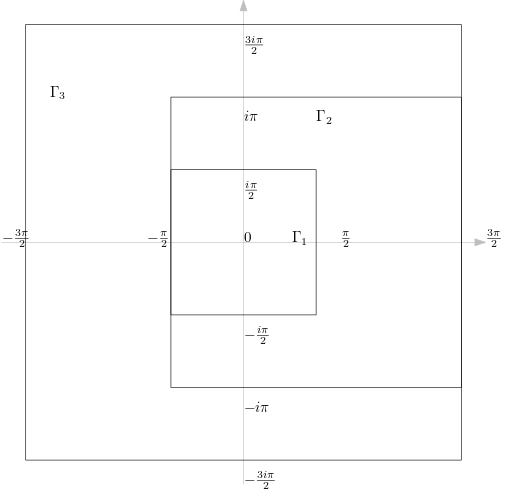
\includegraphics[scale=0.5]{Par20.png}
% 		\label{fig:19.1}
% \end{figure}
\begin{figure}[h!]
		\centering
		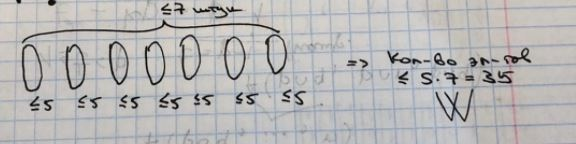
\includegraphics[scale=1]{20}
		\label{fig:19.2}
\end{figure}
Заметим, что $\Gamma_n$~--- квадраты, $l_n = 4\pi n$, $d_n \geq (n-1)\dst
\frac{\pi}{2}$, $\dst \frac{l_n}{d_n}\leq 16$. Значит, система контуров
правильная.
\\
Рассмотрим условия теоремы $7$. На вертикальных границах $\Gamma_n$ $z = \dst
\frac{\pi}{2} + \pi m + iy$. Тогда
\begin{align*}
  & \left| f(z) \right| = \frac{\left| \cos\left( \frac{\pi}{2}+\pi m + iy \right) \right|}{\left| \sin\left( \frac{\pi}{2}+\pi m + iy \right) \right|} = \frac{\left| \sin(iy) \right|}{\left| \cos(iy) \right|} = \frac{\left| e^{-y} - e^y \right|}{\left| e^{-y}+e^y \right|} \leq 1
\end{align*}
Видим, что функция ограничена на них. На горизонтальных границах $\Gamma_n$ $z =
x \pm i \dst \frac{\pi n}{2} = x+iy_n$. Тогда
\begin{align*}
  & \left| f(z) \right| = \frac{\left| e^{-y_n+ix}+e^{y_n-ix} \right|}{\left| e^{-y_n+ix}+e^{y_n-ix} \right|} \leq \frac{\left| e^{-y_n}+e^{y_n} \right|}{\left| e^{-y_n}+e^{y_n} \right|} \leq \frac{ 1+e^{-2\abs{y_n}}}{ 1-e^{-2\abs{y_n}}} \leq 2
\end{align*}
Видим, что функция ограничена на них.
\\
По замечанию $1$ $\dst \frac{\ctg z}{z}$ удовлетворяет условиям теоремы $7$, а
значит, $z = 0$~--- полюс второго порядка, $z_k = \pi k$~--- полюса первого
порядка, и тогда
\begin{align*}
  & \frac{\ctg z}{z} = \frac{\cos z}{z \sin z} = \frac{1 - \dst \frac{z^2}{2!} +\dots}{z^2 - \dst \frac{z^4}{3!}+\dots} = \frac{1}{z^2} +c_0 + c_1z + \dots
\end{align*}
\begin{align*}
  & q_0(z) = \frac{1}{z^2}
\end{align*}
\begin{align*}
  & z_k = \pi k, \ k \neq 0
\end{align*}
Значит,
\begin{align*}
  &  q_k = \frac{\us{\pi k}{\res}\dst \frac{\ctg z}{z}}{z - \pi k} = \frac{1}{\pi k (z - \pi k)}
\end{align*}
\begin{align*}
  & \frac{\ctg z}{z} = \frac{1}{z^2} +\sum_{^{k=-\infty}_{k \neq 0}}^{+\infty}\frac{1}{\pi k (z-\pi k)}
\end{align*}
\begin{align*}
  & \ctg z = \frac{1}{z} +\sum_{^{k=-\infty}_{k \neq 0}}^{+\infty}\frac{z+\pi k -\pi k}{\pi k (z-\pi k)} = \frac{1}{z} +\sum_{^{k=-\infty}_{k \neq 0}}^{+\infty}\left( \frac{1}{\pi k} + \frac{1}{z-\pi k}\right) = \frac{1}{z} +\sum_{k=1}^{\infty}\left( \frac{1}{\pi k} + \frac{1}{z-\pi k} + \frac{1}{-\pi k} + \right. \\
  &\left. \frac{1}{z+\pi k}\right) = \frac{1}{z} +\sum_{k=1}^{\infty}\left( \frac{1}{z-\pi k} + \frac{1}{z+\pi k}\right)
\end{align*}
\section{$\S 20.$ Принцип аргумента. Теорема Руше.}
\theorem
Пусть $f: G \mapsto \CC$
Пусть $G$~--- односвязная облась в $\CC$, $\ogamma$~--- простая замкнута
положительно ориентированная кривая в этой области. Пусть $f: G \mapsto \CC$
регулярна в $G$ за исключением, быть может, полюсов $a_1, \dots, a_k, \dots$,
лежащих внутри $\ogamma$. Пусть на $\ogamma$ нет особых точек $f$. Тогда
справедливо:
\begin{equation}\label{(20.1)}
    \frac{1}{2 i \pi}\int_{\ogamma} \frac{f'(z)}{f(z)}dz = N - P
\end{equation}
где $N$~--- число нулей, $P$~--- полюсов с учетом их порядка (каждый ноль или
полюс считаем такое число раз, каков его порядок)).
\pr
Пусть $b_1, \dots, b_n$~--- нули $f$ внутри $\ogamma$. В силу компактности
ограниченной $\ogamma$ области вместе с кривой и того. что $f(z) \not \equiv 0$,
их конечное число.
\\
Рассмотрим любой нуль $b = b_k$ порядка $m$. Тогда
\begin{align*}
  & f(z) = (z-b)^mh(z), \ z \in B_\varepsilon(b), \ \forall z \in B_\varepsilon(b) \ h(z) \neq 0
\end{align*}
Тогда
\begin{align*}
  & \frac{f'(z)}{f(z)} = \frac{m(z-b)^{m-1}h(z)+(z-b)^mh'(z)}{(z-b)^mh(z)} = \frac{m}{z-b} + \frac{h'(z)}{h(z)}
\end{align*}
и, значит,
\begin{align*}
  & \us{b}{\res}\frac{f'(z)}{f(z)} = m
\end{align*}
Пусть $a_1, \dots, a_p$~--- полюса, их, аналогично, тоже конечное число.
\\
Рассмотрим произвольный полюс $a = a_k$ порядка $l$. Тогда
\begin{align*}
& f(z) = \frac{p(z)}{(z-a)^l}, z \in \os{\circ}{B}_\delta(a), \ \forall z \in \os{\circ}{B}_\delta
(a) \ p(z)\neq 0
\end{align*}
Тогда
\begin{align*}
  & \frac{f'(z)}{f(z)} = \frac{-l}{z-a} + \frac{p'(z)}{p(z)}
\end{align*}
\begin{align*}
  & \us{a}{\res}\frac{f'(z)}{f(z)} = -l
\end{align*}
Отсюда по теореме Коши имеем \eqref{(20.1)}
\corollary (принцип аргумента)
В условии теорем $20.1$
\begin{equation}\label{(20.2)}
  \frac{1}{2\pi} \Delta_{\ogamma}\argt f(z) = N - P
\end{equation}
\pr
Пусть $\ogamma: z = z(t)$, $z(0) = z(1)$, $\ogamma$~--- гладкая замкнутая кривая.
\\
Пусть $\os{\circ}{\Gamma} = f(\ogamma)$, $0 \not \in \os{\circ}{\Gamma}$, $w =
f(z(t))$, $t \in [0;1]$.
\\
Тогда
\begin{align*}
  & \Real \int_{\os{\circ}{\Gamma}}\frac{dw}{w} = \Real \int_{\os{\circ}{\gamma}}\frac{f'(z)}{f(z)}dz = \ln\left| w \right| \Big|_{f(z(1))}^{f(z(0))} = 0
\end{align*}
\begin{align*}
  & \Img \int_{\os{\circ}{\Gamma}}\frac{dw}{w} = \Img \int_{\os{\circ}{\gamma}}\frac{f'(z)}{f(z)}dz = \Delta_{\ogamma}\argt f(z)
\end{align*}
\begin{align*}
  & \int_{\os{\circ}{\gamma}}\frac{f'(z)}{f(z)}dz = i\Delta_{\ogamma}\argt f(z)
\end{align*}
Тогда из \eqref{(20.1)} очевидно следует \eqref{(20.2)}.